\documentclass{article}

\usepackage[fleqn]{amsmath}
\usepackage{amssymb}
\usepackage{hyperref}
\usepackage{url}
\usepackage{graphicx}
\usepackage{geometry}
\usepackage{babel}
\usepackage{enumitem}
\usepackage{parskip}
\usepackage{chemfig}
\usepackage{pdfpages}
\usepackage{xcolor}
\usepackage{tikz}
\usepackage{fancybox}
\usepackage{makecell}
\usepackage{pgfplots}
\usepackage{soul}
\usepackage{ulem}
\usepackage{wrapfig}
\usepackage{subcaption}
\usepackage[T1]{fontenc}
\usepackage{pgfplots}
\usepackage{esvect}
\usetikzlibrary{arrows}
\usetikzlibrary{decorations.pathreplacing}
\pgfplotsset{compat=1.17}

\geometry{
    a4paper,
    total={170mm, 257mm},
    left=20mm,
    top=20mm
}

\hypersetup{
    colorlinks=true,
    linkcolor=black,
    urlcolor=blue,
    pdftitle={Mathematics 1A}
}

\newcommand{\figbox}[1]{ 
    \begin{figure*}[ht!]        
        \begin{center}            
            \fbox{#1}        
        \end{center}    
    \end{figure*}
}

\newcommand{\wrapfill}{
    \par
    \ifnum \value{WF@wrappedlines} > 0
        \addtocounter{WF@wrappedlines}{-1}%
        \null\vspace{
            \arabic{WF@wrappedlines}
            \baselineskip
        }
        \WFclear
    \fi
    \phantom{}
}

\newcommand{\difference}{\,\backslash\,}
\newcommand{\rem}{\underline{Remark}: }
\newcommand{\nots}{\underline{Notation}: }
\newcommand{\prf}{\underline{Proof}: }
\newcommand{\exs}{\underline{Example}: }
\newcommand{\defs}{\underline{Definition}: }
\newcommand{\sht}{\ |\ }

% === TEXT ===
\title{\textbf{Mathematics 1A \\ HSLU, Semester 1}}
\author{Matteo Frongillo}

\begin{document}

\maketitle
\tableofcontents
\pagebreak

\part{Week 1}
\section{The set theory}
\subsection{Definition of a set}
A set is a collection of objects or elements.

\rem{The collection of all sets is not a set.}

\subsection{Logical symbols}
\subsubsection{Definition}
Braces and the definition symbol ``$:=$'' are used to define a set giving all its elements:
\figbox{$A:=\left\{a,b,c,d,e\right\}$}

\subsubsection{Equal}
In this case, the equal symbol means that the set $A$ is equal to the set $B$:
\figbox{$A=B$}

\subsubsection{Belongs to}
The symbols $\in$ and $\ni$ describe an element which is part of the set:
\figbox{$a \in A \Longleftrightarrow A \ni a$}

\subsubsection{Does not belong to}
The symbols $\notin$ mean that an element does not belong to the set:
\figbox{$f \notin A$}

\subsubsection{Inclusion and contains}
The symbols $\subset$ and $\supset$ mean that a set has another set included in its set:
\figbox{$\mathbb{N} \subset \mathbb{Z} \Longleftrightarrow \mathbb{Z} \supset \mathbb{N}$}

\subsubsection{For all/any}
The symbol $\forall$ means that we are considering any type of element:
\figbox{$\forall x \in \mathbb{R},\ x>0$}

In this case, we've defined a new set.

\newpage
\subsubsection{Implication}
The symbol $\Rightarrow$ means that by setting a rule, we imply an event or an action:
\figbox{if $x=1 \Longrightarrow x \in \mathbb{N}$, but if $x \in \mathbb{N}$ we do not know if $x=1$}

With the implication, it is \underline{sufficient} to claim action "A" in order to claim action "B".

\subsubsection{Inference}
The symbol $\Leftarrow$ means that by having an event or an action, we have a rule.
\figbox{$x \in \mathbb{R}^+ \Longleftarrow x > 0$}

With the inference, it is \underline{necessary} to have claim the action ``A'' in order to have claim the action ``B''


\subsubsection{If and only if}
The symbol $\Leftrightarrow$ means that two events happen simultaneously (double implication):
\figbox{$x \in \mathbb{N},\ x \neq 0 \Longleftrightarrow x \in \mathbb{N}^*$}

\exs{}

$x=2 \Longleftrightarrow x^2-4x+4=0$

\prf{}

$x=2 \Rightarrow (x-2)=0 \Rightarrow (x-2)^2=0\cdot(x-2) \Rightarrow x^2-4x+4=0$

This happens \textbf{because} $x=2$

\subsection{Numerical sets}
\begin{itemize}
    \item $\mathbb{N} :=$ Natural numbers (including 0);
    \item $\mathbb{Z} :=$ Integer numbers;
    \item $\mathbb{Q} :=$ Rational numbers;
    \item $\mathbb{R} := \text{Real numbers} := \mathbb{Q} \cup \left\{\text{irrational numbers}\right\}.$
\end{itemize}

\nots{The ``$^*$'' symbol means that the set does not include 0.}

\subsubsection{Inclusion of sets}
\figbox{$\mathbb{N} \subset  \mathbb{Z} \subset \mathbb{Q} \subset \mathbb{R} \subset \mathbb{C}$}

$
    B := \left\{\pi, 1,-1,0\right\}; \\
    C := \left\{\pi, 1\right\}; \\
    D := \left\{\pi\right\}.
$

Then we write some examples: $\pi \in B,\ D \subset B,\ C \subset B,\ B \not\subset C,\ 0 \in B,\ 0 \notin C$.

\newpage
\section{Intervals in the real line}
Intervals describe what happens between two or more elements.

\subsection{Examples}
\subsubsection{Interval sets}
We have 4 cases:
\begin{itemize}
    \item $(a,b) = \left\{\forall x \in \mathbb{R} \sht a<x<b\right\}$;
    \item $\left[a,b\right) = \left\{\forall x \in \mathbb{R} \sht a\leq x<b\right\}$;
    \item $\left(a,b\right] = \left\{\forall x \in \mathbb{R} \sht a<x\leq b\right\}$;
    \item $\left[a,b\right] = \left\{\forall x \in \mathbb{R} \sht a\leq x\leq b\right\}$.
\end{itemize}

\nots{$a$ and $b$ are often called the ``end points'' of the interval;\\}

\subsubsection{Graphical examples}
$\forall x \in \mathbb{R},\ x \in \left[a,b\right]$
\begin{center}
    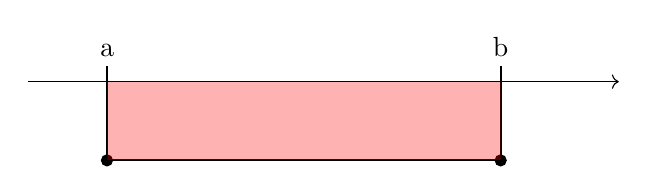
\begin{tikzpicture}
        %number line
        \draw[-] (-4,0) -- (3,0);
        \draw[thick] (-3,-0.2) -- (-3,0.2);
        \draw[thick] (2,-0.2) -- (2,0.2);
        
        %interval
        \draw[thick] (-3,-1) -- (2,-1);
        \draw[thick] (-3,0) -- (-3,-1);
        \draw[thick] (2,0) -- (2,-1);
        \filldraw[black] (-3,-1) circle (2pt);
        \filldraw[black] (2,-1) circle (2pt);
        
        %points
        \node[above] at (-3,0.2) {a};
        \node[above] at (2,0.2) {b};
        
        %arrow
        \draw[->] (3,0) -- (3.5,0);

        %area
        \filldraw [fill=red, draw=black, opacity=0.3] (-3,0) rectangle (2,-1);
    \end{tikzpicture}
\end{center}

\section{The extended line}
In the real line $\mathbb{R}$ we add $\pm \infty$.

\paragraph{Real line:} $(-\infty, +\infty) = \mathbb{R}$ 

\paragraph{Extended real line:} $\left[-\infty, +\infty\right] = \overline{\mathbb{R}}$

\vspace*{.5cm}
\begin{center}
    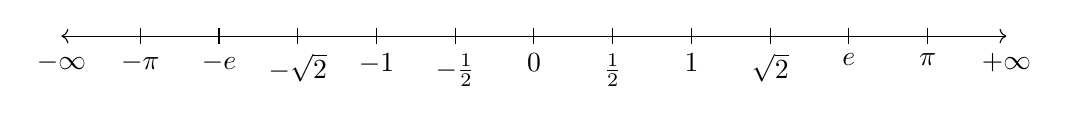
\begin{tikzpicture}
        \draw[->] (0,0) -- (6,0);
        \draw[<-] (-6,0) -- (0,0);

        \foreach \x/\label in {-5/{$-\pi$}, -4/{$-e$}, -3/{$-\sqrt{2}$}, -2/{$-1$}, -1/{$-\frac{1}{2}$}, 0/{$0$}, 1/{$\frac{1}{2}$}, 2/{$1$}, 3/{$\sqrt{2}$}, 4/{$e$}, 5/{$\pi$}} {
            \draw (\x,0.1) -- (\x,-0.1) node[below] {\label};
        }
        \node[below] at (-6,-0.1) {$-\infty$};
        \node[below] at (6,-0.1) {$+\infty$};
    \end{tikzpicture}
\end{center}

\rem{$\pm \infty \notin \mathbb{R}$}

\subsection{Properties}
\figbox{$\forall x \in \mathbb{R} \ \sht \ \infty > x \ \sht \ -\infty < 0$}

\subsection{Operation in the extended line}
If $a,b \in \mathbb{R}$, then $a+b,\; a-b,\; a\cdot b,\; \frac{a}{b} \text{ (with } b\neq 0 )$ stay the same

\subsubsection{Additions}
Let $\forall a \in \mathbb{R}$:
\begin{itemize}
    \item $a+\infty := \infty$;
    \item $a-\infty := -\infty$;
    \item $+\infty + \infty := +\infty$;
    \item $-\infty - \infty := -\infty$;
    \item $+\infty - \infty :=$ undefined.
\end{itemize}

\subsubsection{Moltiplications}
Let $\forall a \in \mathbb{R}$:
\begin{itemize}
    \item $+\infty \cdot +\infty := +\infty$;
    \item $-\infty \cdot +\infty := -\infty$;
    \item $-\infty \cdot (-\infty) := \infty$;
    \item $a \cdot \infty := \begin{cases}
        a > 0 &+\infty\\
        a < 0 &-\infty\\
        a = 0 & \text{undefined}
    \end{cases}$
    \item $a \cdot (-\infty):= \begin{cases}
        a > 0 &-\infty\\
        a < 0 &+\infty\\
        a = 0 &\text{undefined}
    \end{cases}$
    \item $\frac{a}{+\infty}=\frac{a}{-\infty} := 0$;
    \item $\frac{+\infty}{a}:= \begin{cases}
        a > 0 &+\infty\\
        a < 0 &-\infty\\
        a = 0 &+\infty
    \end{cases}$
    \item $\frac{-\infty}{a}:= \begin{cases}
        a > 0 &-\infty\\
        a < 0 &+\infty\\
        a = 0 &-\infty
    \end{cases}$
    \item $\frac{\infty}{\infty}:=$ undefined.
\end{itemize}

\section{Intervals including $\pm \infty$}
Intervals describe what happens between two or more elements, including $\pm \infty$.
\subsection{Examples}
\subsubsection{Interval sets}
Let $a \in \mathbb{R}$, then:
\begin{itemize}
    \item $(-\infty,a)=\left\{\forall x \in \mathbb{R} \sht x < a\right\}$;
    \item $(a, +\infty)=\left\{\forall x \in \mathbb{R} \sht x > a\right\}$;
    \item $(-\infty, a]=\left\{\forall x \in \mathbb{R} \sht x \leq a\right\}$;
    \item $[a,+\infty]=\left\{\forall x \in \mathbb{R} \sht x \geq a\right\}$;
    \item $(-\infty,+\infty)=\mathbb{R}$;
    \item $[-\infty,+\infty]=\overline{\mathbb{R}}$.
\end{itemize}

\subsubsection{Graphical examples}
$\forall x \in \mathbb{R},\ x \in\ \left[a,b\right]\ \cup\ \left] c, +\infty\right[$

\begin{center}
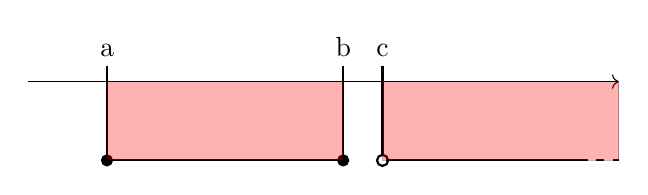
\begin{tikzpicture}
    %number line
    \draw[-] (-3,0) -- (4,0);
    \draw[thick] (-2,-1) -- (-2,0.2);
    \draw[thick] (1,-1) -- (1,0.2);
    \draw[thick] (1.5,-0.95) -- (1.5,0.2);
    
    %intervals
    \draw[thick] (-2,-1) -- (1,-1);
    \filldraw[black] (-2,-1) circle (2pt);
    \filldraw[black] (1,-1) circle (2pt);
    \draw[thick] (1.55,-1) -- (4,-1);
    \draw[thick, dashed] (4,-1) -- (4.5,-1);
    \draw[thick] (1.5,-1) circle (2pt);
    
    %points
    \node[above] at (-2,0.2) {a};
    \node[above] at (1,0.2) {b};
    \node[above] at (1.5,0.2) {c};
    
    %arrow
    \draw[->] (4,0) -- (4.5,0);

    %area
    \filldraw [fill=red, draw=black, opacity=0.3] (-2,0) rectangle (1,-1);
    \filldraw [fill=red, draw=black, opacity=0.3] (1.5,0) rectangle (4.5,-1);
\end{tikzpicture}
\end{center}
\vspace*{.5cm}
\nots{The union of two or more intervals where $x \in \mathbb{R}$
is denoted by the symbol $\cup$.}

\newpage
\section{Union and Intersection}
\subsection{Logical symbols AND, OR and NOT}
\begin{itemize}
    \item $\land$ = AND;
    \item $\lor$ = OR;
    \item $\lnot$ = NOT.
\end{itemize}

\subsection{Universe symbol}
The symbol $\bigcup :=$ Universe describes a big set which contains all sets involved
in our discussions (not always).

Let $A,B$ be two sets $\left[A \subset \bigcup,\ B \subset \bigcup\right]$. Then:
\begin{itemize}
    \item $A \cup B =$ union of $A$ and $B \Longrightarrow \left\{\forall x \in \bigcup \sht x \in A \lor x \in B\right\}$;
    \item $A \cap B =$ intersection between $A$ and $B \Longrightarrow \left\{\forall x \in \bigcup \sht x \in A \land x \in B\right\}$.
\end{itemize}

\subsection{\color{red}{Venn diagram}}
\subsubsection{Union $A \cup B$}
\figbox{
    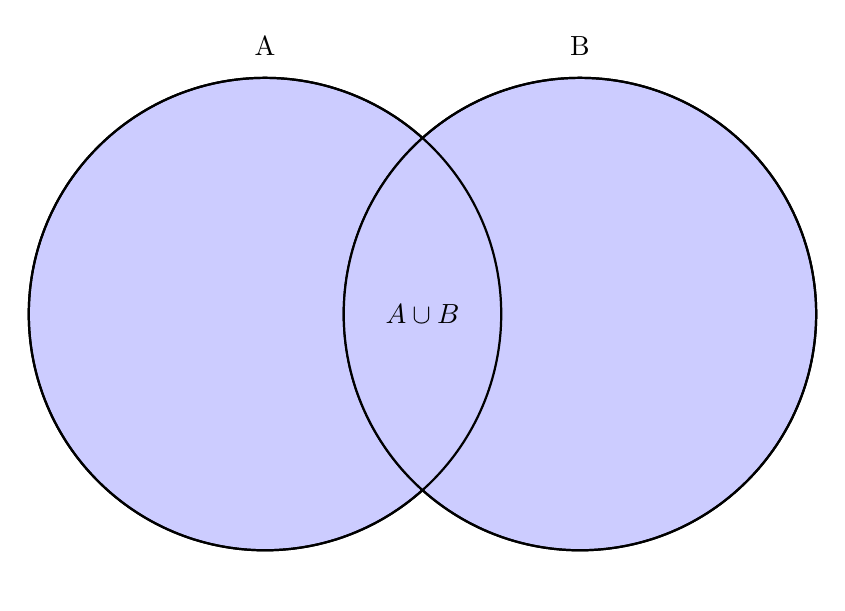
\begin{tikzpicture}[scale=2]
        \draw[thick, fill=blue!20] (2, 2) circle (1.5);
        \draw[thick, fill=blue!20] (4, 2) circle (1.5);
        
        \begin{scope}
            \clip (2, 2) circle (1.5);
            \fill[white] (4, 2) circle (1.5);
            \clip (2, 2) circle (1.5);
            \fill[blue!20] (4, 2) circle (1.5);
        \end{scope}

        \draw[thick] (2, 2) circle (1.5);
        \draw[thick] (4, 2) circle (1.5);
        
        \node at (2, 3.7) {A};
        \node at (4, 3.7) {B};
        
        \node at (3, 2) {\(A \cup B\)};
        
        \node at (3, 0.35) {};

        \node[overlay] at (0.2,3.75) {\(\bigcup\)};
    \end{tikzpicture}
}

\subsubsection{Intersection $A \cap B$}
\figbox{
    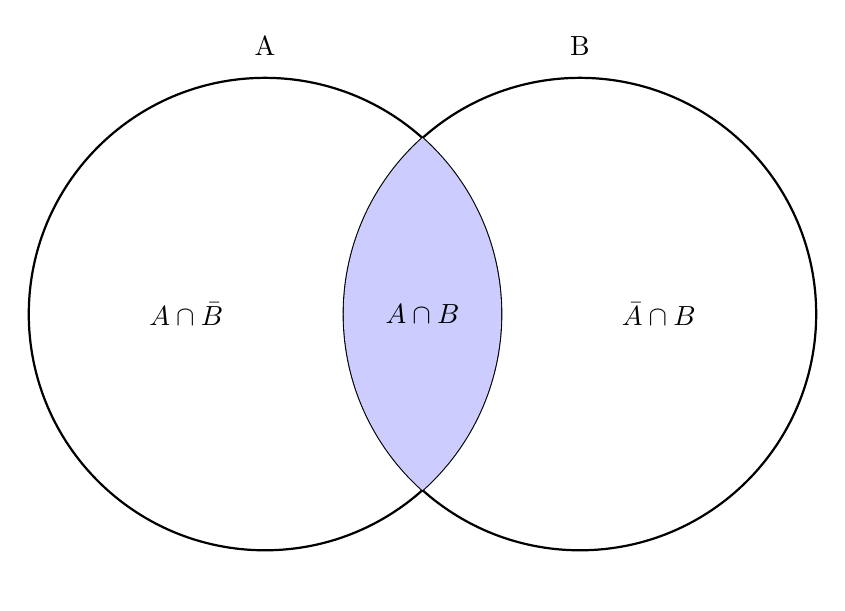
\begin{tikzpicture}[scale=2]
        
        \draw[thick] (2, 2) circle (1.5);
        \draw[thick] (4, 2) circle (1.5);
        \begin{scope}
            \clip (2, 2) circle (1.5);
            \fill[blue!20] (4, 2) circle (1.5);
        \end{scope}
        
        \node at (2, 3.7) {A};
        \node at (4, 3.7) {B};
        
        \node at (1.5, 2) {\(A \cap \bar{B}\)};
        \node at (4.5, 2) {\(\bar{A} \cap B\)};
        \node at (3, 2) {\(A \cap B\)};
        
        \node at (3, 0.35) {};

        \node[overlay] at (0.2,3.75) {\(\bigcup\)};
    \end{tikzpicture}
}

\newpage
\subsubsection{The complementary element $\overline{A}$}
$1-A = \overline{A}$

\begin{figure}[ht!]
    \begin{center}
            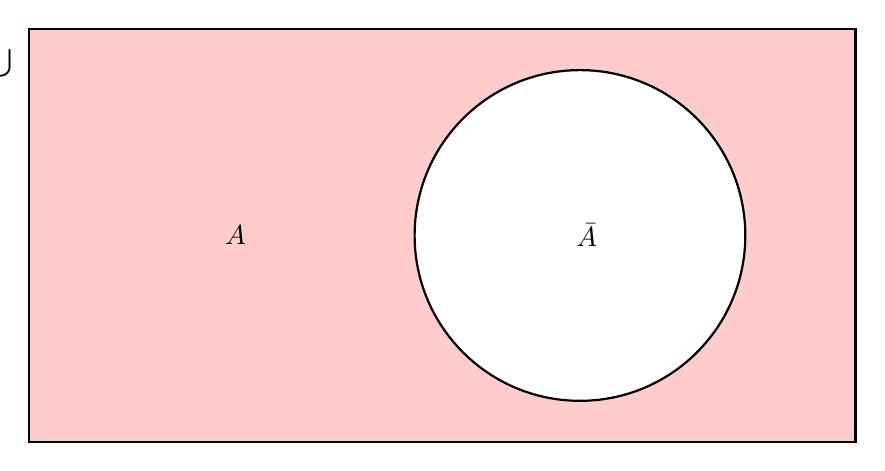
\begin{tikzpicture}[scale=1.75]
                
                \fill[red!20] (0, 0) rectangle (6, 3);
                \draw[thick] (0, 0) rectangle (6, 3);
        
                \fill[white] (4, 1.5) circle (1.2);
                \draw[thick] (4, 1.5) circle (1.2);
                
                \node at (1.5, 1.5) {\(A\)};
                \node at (4.05, 1.5) {\(\bar{A}\)};
                            
                \node[overlay] at (-0.2,2.75) {\(\bigcup\)};
            \end{tikzpicture}
    \end{center}
\end{figure}

\subsubsection{Difference between sets}
$A \difference B = \left\{\forall x \in \bigcup \sht x \in A,\ x \notin B\right\}$

COLORARE TUTTO A PARTE $A \cup B$!!
\figbox{        
    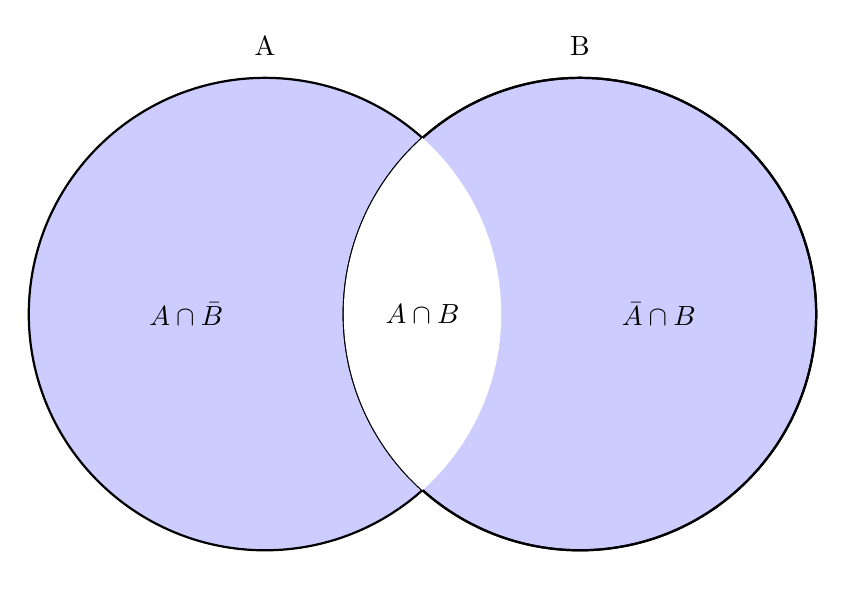
\begin{tikzpicture}[scale=2]
        \draw[thick, fill=blue!20] (2, 2) circle (1.5);
        \draw[thick, fill=blue!20] (4, 2) circle (1.5);
        \draw[thick] (4, 2) circle (1.5);
            
        \begin{scope}
            \clip (2, 2) circle (1.5);
            \fill[white] (4, 2) circle (1.5);
        \end{scope}
        
        \node at (2, 3.7) {A};
        \node at (4, 3.7) {B};
        
        \node at (1.5, 2) {\(A \cap \bar{B}\)};
        \node at (4.5, 2) {\(\bar{A} \cap B\)};
        \node at (3, 2) {\(A \cap B\)};
        
        \node at (3, 0.35) {};

        \node[overlay] at (0.2,3.75) {\(\bigcup\)};
    \end{tikzpicture}
}

\newpage
\subsubsection{Empty set $\emptyset$}
$\emptyset :=$ the set containing zero elements:
$A \cup B = \emptyset$

\defs{$A \bigtriangleup B = (A \difference B) \cup (B \difference A)$}

\section{The absolute value function}
The absolute value is an operator which turns positive the sign of the result of the function.

Let $x \in \mathbb{R}$, then:
\figbox{$|x|=\begin{cases}
    x \text{\quad if} &x \geq 0\\
    x \text{\quad if} &-x \leq 0
\end{cases}$}

\subsection{Graph of absolute value functions}
Let's plot the function $y=|x|$:
\begin{figure}[ht!]
    \centering
    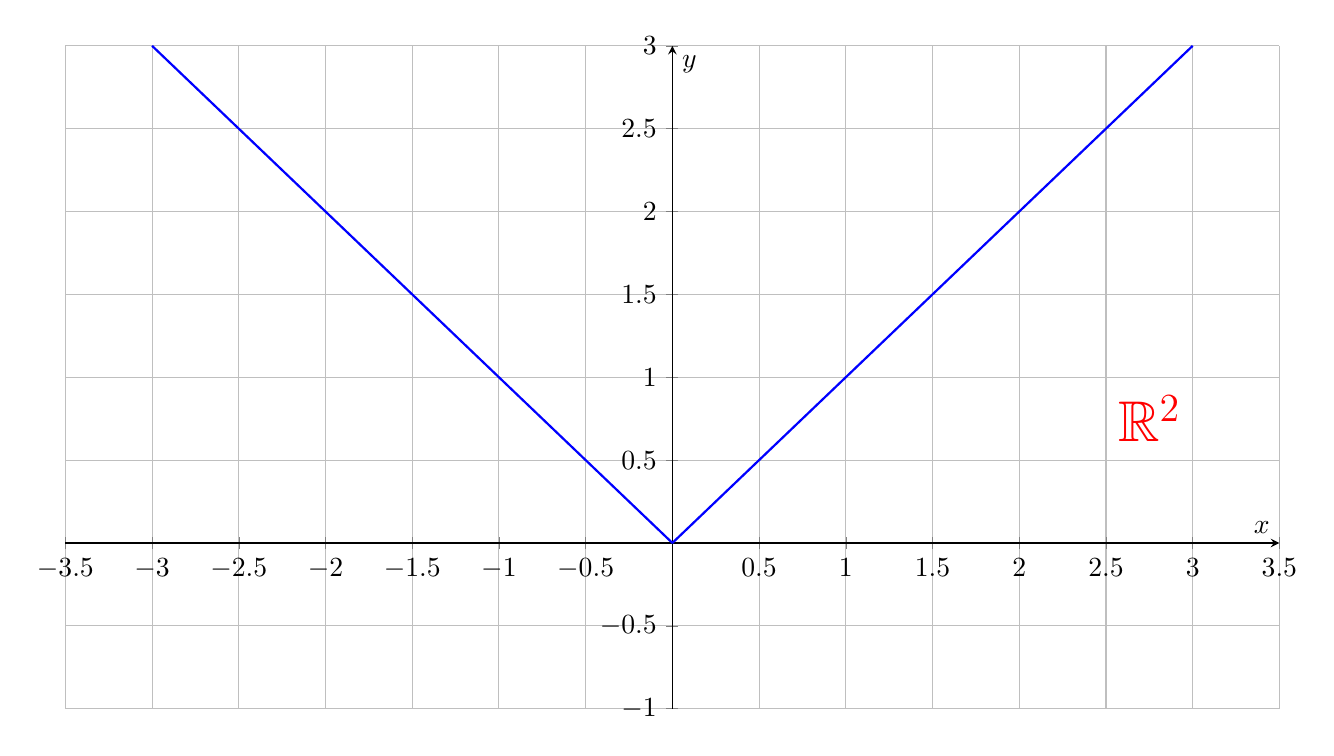
\begin{tikzpicture}
        \begin{axis}[
            axis lines = middle,
            xlabel = {$x$},
            ylabel = {$y$},
            domain=-3:3,
            samples=1500,
            xmin=-3.5, xmax=3.5,
            ymin=-1, ymax=3,
            grid=major,
            width=17cm, height=10cm
        ]
            \addplot[blue, thick] {abs(x)};
            \node[red] at (2.75,.75) {\huge $\mathbb{R}^2$};
            \end{axis}
    \end{tikzpicture}
\end{figure}

\subsection{Properties}
Let $a,b \in \mathbb{R}$, then:
\begin{itemize}
    \item $|a\cdot b|=|a| \cdot |b|$;
    \item $|\frac{a}{b}|= \frac{|a|}{|b|} \quad$ for $b \neq 0$;
    \item $|a\pm b| \neq |a|\pm |b|$.
\end{itemize}

\subsection{Triangolar inequalities}
Let $a,b \in \mathbb{R}$, then:
\figbox{\begin{minipage}{0.135\textwidth}
    \begin{center}
        $|a|+|b| \geq |a+b|$\\
        $|a|-|b| \leq |a-b|$ 
    \end{center}
\end{minipage}
}





\end{document}
